\documentclass[12pt]{article}
\usepackage[T2A]{fontenc}

\usepackage{amssymb,amsthm,amsmath}
\usepackage{graphicx}

\usepackage{eso-pic}

\usepackage{graphicx}

\newcommand\BackgroundPic{%
\put(-25,0){%
\parbox[b][\paperheight]{\paperwidth}{%
\vfill \centering
\includegraphics[width=1.05\paperwidth%,height=\paperheight%,
%keepaspectratio
]{picts/capa}%
\vfill }}}

\tolerance =10000

\textwidth=17cm \oddsidemargin=-5mm \topmargin=-20mm
\textheight=25cm
\renewcommand{\baselinestretch}{1.5}

\begin{document}

%\AddToShipoutPicture*{\BackgroundPic}

\vskip 1cm {\Huge Makar Plakhotnyk}

\vskip 1cm {\huge Planilh\~ao}

{\Large \vskip 1cm \centerline{Projeto de curso}

\centerline{Programa\c{c}\~ao orientada objetos}

%\vskip 1cm
\begin{flushright}prof. Jos\'e Paulo
Ciscato\end{flushright}}

\vskip 16cm \centerline{S\~ao Paulo, 2020}

\thispagestyle{empty}

\newpage

%\pagecolor{blue}

\tableofcontents

\thispagestyle{empty}

\newpage

\setcounter{page}{1}

\section{Introdu\c{c}\~ao}

O assunto principal desse programa \'e dar para usuario um auxilio
de construir um planilha com diagrama de fluxo (fluxogramma).

\begin{figure}[h]
\begin{center}
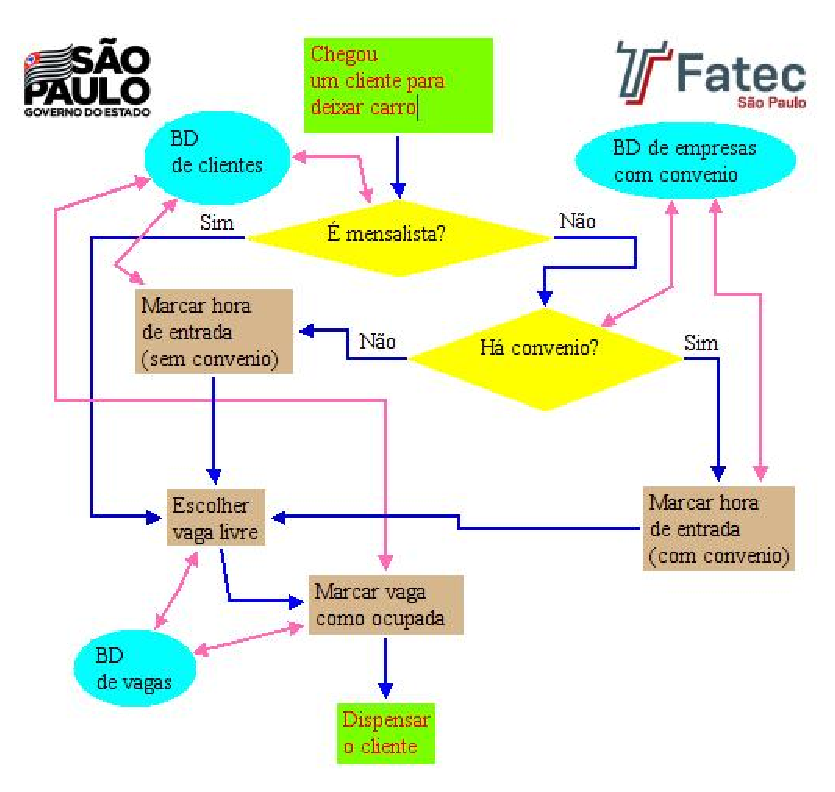
\includegraphics{image-07}
\end{center}
\caption{Diagrama de fluxo}\label{fig-01}
\end{figure}

No Fig.~\ref{fig-01} temos um diagrama, que construimos na \'aula
de IES-100 com professor Brnice, resolvendo uma das tarefas dele.
Esse trabalho deu um motivo para prepara um programa em java, que
simplifica \'a constru\c{c}\~ao de diagramas desse tipo.

\newpage
\section{Descri\c{c}\~ao de programa}





\subsection{Funcionamento}

\begin{figure}[htb]
\begin{center}
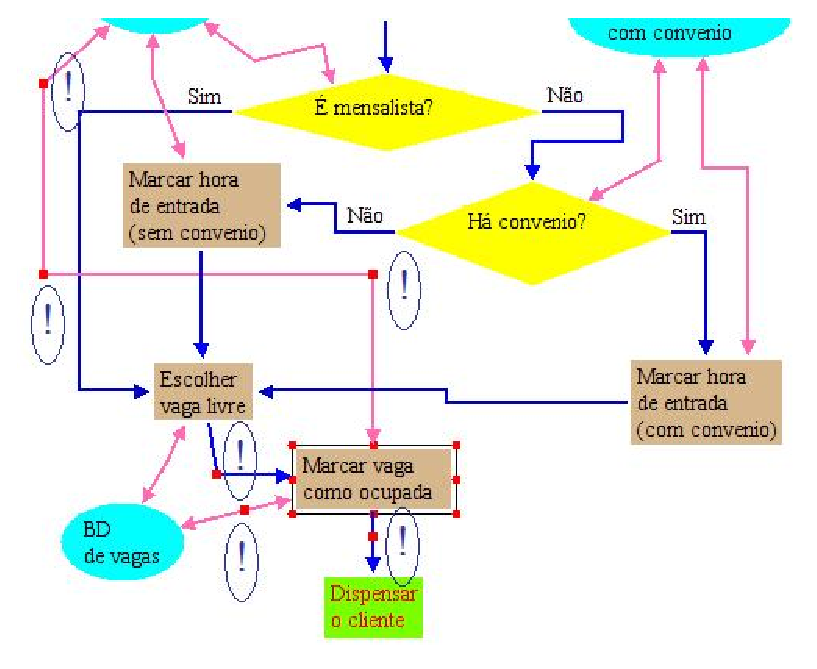
\includegraphics{image-01}
\end{center}
\caption{Active text element}\label{im-01}
\end{figure}


\begin{figure}[htb]
\begin{center}
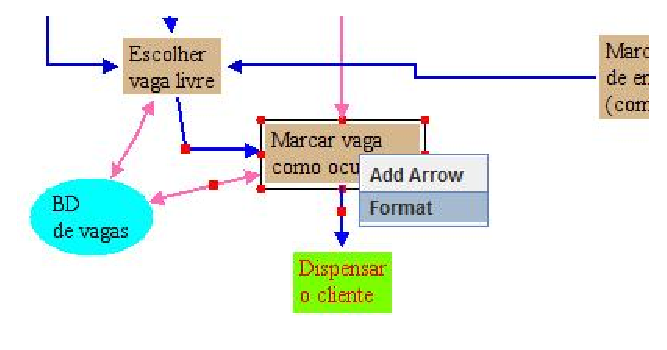
\includegraphics{image-02}
\end{center}
\caption{Text element rClick}\label{im-02}
\end{figure}


\begin{figure}[htb]
\begin{center}
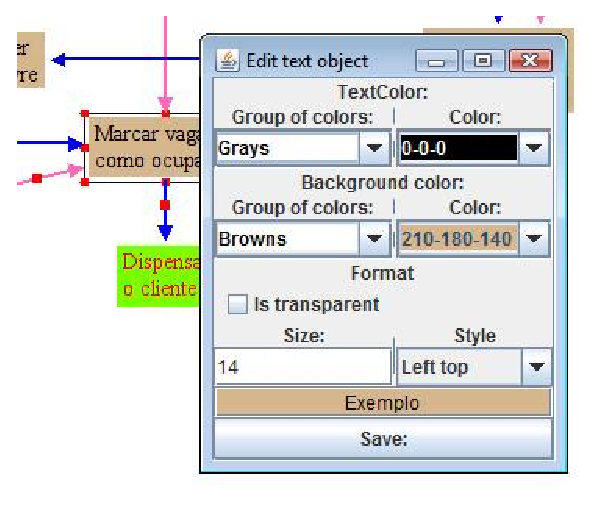
\includegraphics{image-03}
\end{center}
\caption{Text element propriedades}\label{im-03}
\end{figure}

\begin{figure}[htb]
\begin{center}
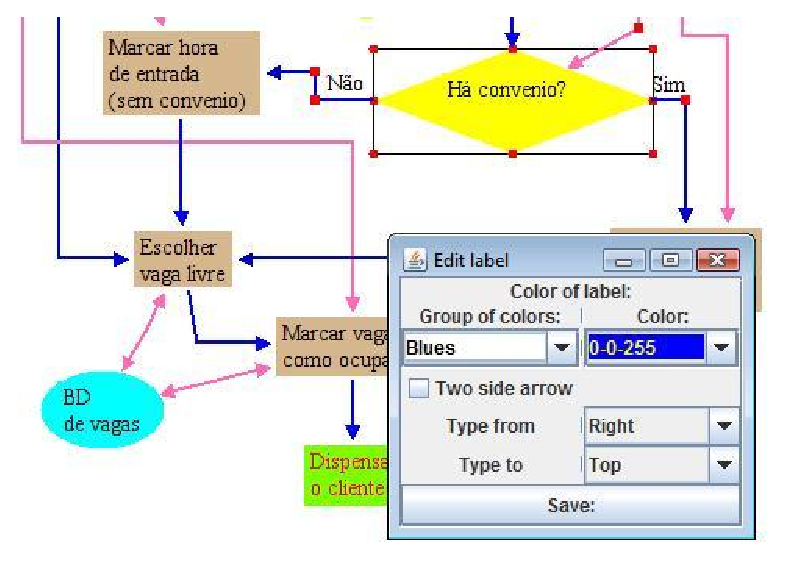
\includegraphics{image-04}
\end{center}
\caption{Label element propriedades}
\end{figure}

\begin{figure}[htbp]
\begin{minipage}[h]{0.45\linewidth}
\begin{center}

\includegraphics[width=0.95\linewidth]{image-11}
\centerline{a. Imagem n\~ao ativa}\end{center}
\end{minipage}
\hfill
\begin{minipage}[h]{0.45\linewidth}
\begin{center}

\includegraphics[width=0.95\textwidth]{image-12}
\centerline{b. Imagem ativa]}\end{center}
\end{minipage}
\hfill \caption{Imagens} \label{fig:19ab}
\end{figure}


A diagrama no Fig.~\ref{fig-01} \'e editavel no sentido, que
interface permita alterar os posi\c{c}\~oes de elementos de
diagrama, testo, formato, flechas etc.






Depois de 1 click no elemento de diagrama qualquer, esse elemento
``ativa-ce'' (veja Fig.~\ref{im-01}). Essa ativa\c{c}\~ao permite
alterar a posi\c{c}\~ao de elemento, posi\c{c}\~oes de quebras de
flechas, formato de imagem e de fleshas.


\begin{figure}[htb]
\begin{center}
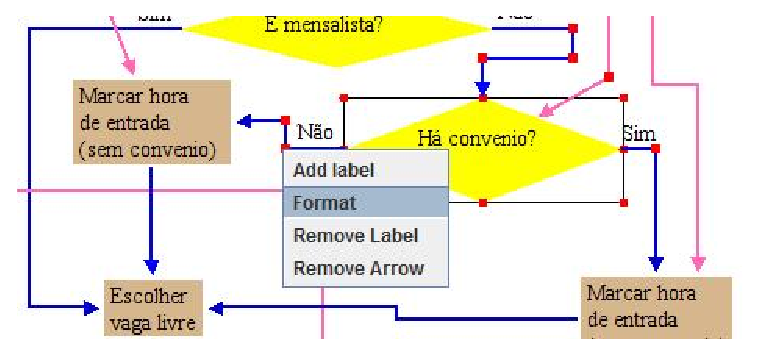
\includegraphics{image-05}
\end{center}
\caption{Label element RClick}
\end{figure}

Com um click de mouse direita no \'area de texto aparece um menu
(veja Fig.~\ref{im-02}), que permita escolher edi\c{c}\~ao de
formato, ou adiciopnar uma flecha desse elemento para um outro
elemento da planilha. Tamb\'em ha uma possibilidade de addicionar
uma flecha para um outro objeto de texto.

A janela de edi\c{c}\~ao de elemento de testo est\'a dado no
Fig~\ref{im-03}. Esse interface permite alterar um cor de fone,
cor de background, tamanho de fonte, se texte \'e transparente, e
posi\c{c}\~ao de testo dentro de objeto (a esqueda, a direita, de
centro etc.).

\begin{figure}[htbp]
\begin{minipage}[h]{0.45\linewidth}
\begin{center}
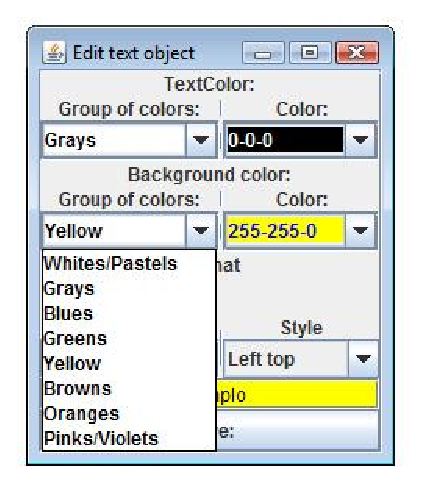
\includegraphics[width=0.95\linewidth]{image-13}
\centerline{a. Grupos de cores}\end{center}
\end{minipage}
\hfill
\begin{minipage}[h]{0.45\linewidth}
\begin{center}
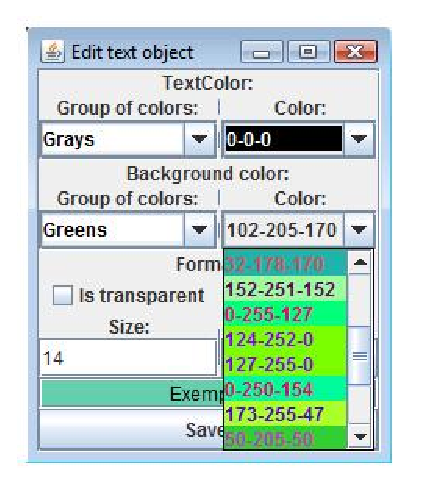
\includegraphics[width=0.95\textwidth]{image-14}
\centerline{b. RGB-cor]}\end{center}
\end{minipage}
\hfill \caption{Edi\c{c}\~ao de cor} \label{fig:13-14}
\end{figure}

\begin{figure}[htb]
\begin{center}
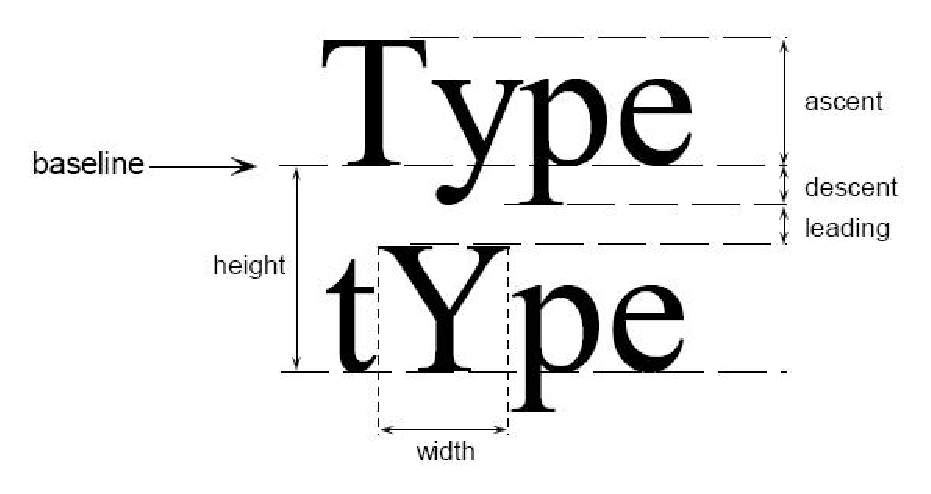
\includegraphics{image-15}
\end{center}
\caption{Parametros de font tipografico}
\end{figure}

\begin{figure}[htb]
\begin{center}
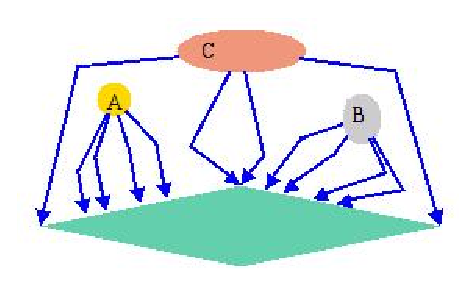
\includegraphics{image-16}
\end{center}
\caption{Formas de flechas relatado com losango}
\end{figure}

\subsection{O que fazer?}

Assim, para preparar o programa planejada, vamos dividir o
trabalho preparatorio para pares de aprendizagem de itens
seguintes:

1. Como, usando Java, \'e possivel alterar uma posi\c{c}\~ao de
objeto de JPanel. Por exemplo, temos Jlabel, ou JTextArea sobre
JPane, usuario aperta mouse, e lo movimenta; queremos movimentar o
nosso obj\'eto tamb\'em. Mesmo quest\~ao sobre alterar tamanho de
objeto.





2. Como desenhar objetos ``com geometria complicada'', por
exemplo: elipce  com testo; losango; recrangulo com angulos
redondos etc.? Os objetos de edi\c{c}\~ao de testo pardr\~ao s\~ao
rectangular, mas como \'e possivel desenvolvel algo um pouco mais
avansado?

3. Como desenhar linhas, flechas, curvas qualquer sobre JPanel?







4. Como mexer com fonts em Java? Por exemplo, como \'e alerar um
font de JTextArea (ou objeto similar) de Times New Roman para
Areal, Verdana etc.? O que \'e fonte negrito, it\'alico se existe
em Java? Tamanho de fonte? Qual \'e i n\'ivel de dificuldade para
mexer com ``tudo isto'', e o que devemos aprender?

5. Como salvar planilha, que ser\'a desenvolvida? Claro, que vamos
desenvolver algum formato proprio, e salvar os rascunhos nesse
formato. Mas usu\'ario deve salvar o resulado final em algum
formato compart\'ivel com os formatos conjecidos. Uma op\c{c}\~ao
(n\~ao a melhor) \'e salvar imagem; outra op\c{c}\~ao \'e slvar
resultado para um arquivo pdf. Devemos aprender fazer sada dessas
op\c{c}\~oes.


\section{Java}



\subsection{Movimentar objetos}

Figura~\ref{im-09} comtem uma janela de programa na
execu\c{c}\~ao. No terminologia de Java a janela se chama
``frame''. De baixo de menu est\'a uma parte de janela (frame),
para onde podemos colocar-la outros elementos. A pr\'atica mais
commun de usar frame com elementos \'e colocar uma panela no
frame, e depois colocar os elementos para panela.

O classe mais commun para usar para texto com muitas linhas \'e
JTextArea. Assim, o programa de Figura~\ref{im-09} tem 5
elementos: JFrame, JScrollPane, JMenu, JPanel, JTextArea, e
orgniza\c{c}\~ao deles est\'a mostrada na Fig.~\ref{im-10}.

\begin{figure}[htbp]
\begin{center}
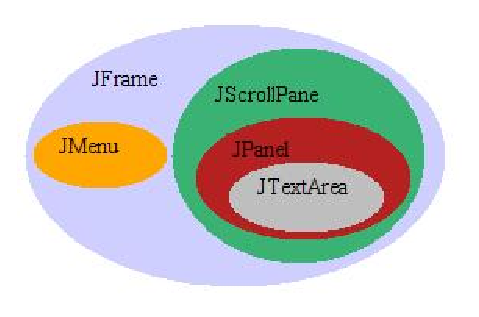
\includegraphics{image-10}
\end{center}
\caption{Elements of a frame}\label{im-10}
\end{figure}

Cada elemento tem sua posi\c{c}\~ao: um par de n\'imeros inteiros
n\~ao negativos, digamos $(x,\, y)$, que \'e uma coordenada de
canto cima esquerda corespondendene de outro objeto, onde est\'a
colocado o dado.

\begin{figure}[htbp]
\begin{center}
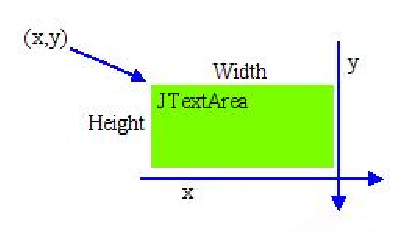
\includegraphics{image-08}
\end{center}
\label{im-08} \caption{Text Area}
\end{figure}



\section{Paper and fonts}

\begin{figure}[htb]
\begin{center}
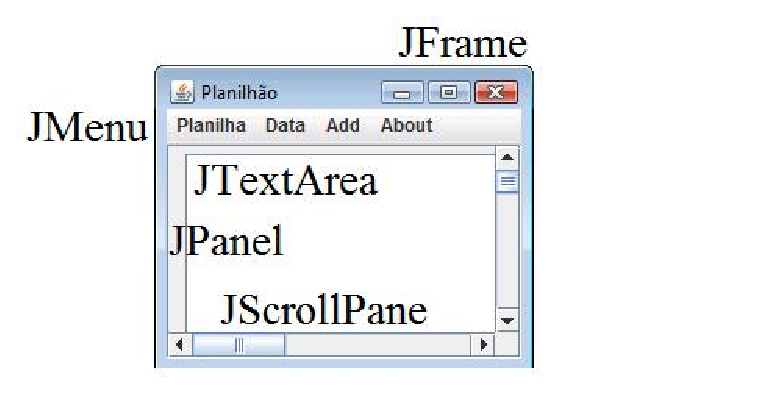
\includegraphics{image-09}
\end{center}
\caption{Structure of a frame}\label{im-09}
\end{figure}

\subsection{Measures, which are used for fonts, pages and
paragraphs}

One of the most common sizes of paper is called ``A4''. It means
that measures of page are:

\begin{center}
A4: $\begin{array}{ll} \text{210mm x 297mm, or}\\
\text{8.27in x
11.69in}\end{array}$
\end{center}

The former measure is millimeters, and the last is inches. The
conversion of inch to meters can be done, using

\centerline{1 inch = 2.54 centimeters.}

An important characteristic of printers and scanners is the number
of dots, which the print (or recognize) per inch, abbreviated as
DPI (dot per inch). This measure is called (print, or scan)
resolution. For example, if the resolution is 72 DPI, then A4
paper contains $$\begin{array}{ll}\text{width: 8.27in = 8.27*72pt
}\approx 595,44 \text{pt}\approx 595\text{pt}\\
\text{height: 11.69in =11.69*72pt}\approx 841,68\text{pt} \approx
842\text{pt}
\end{array}$$

Standard ISO A4 paper dimensions are:




Equivalent A4 paper dimensions in pixels at 300 DPI and 72 DPI
respectively are:

    2480 pixels x 3508 pixels (print resolution)
    595 pixels x 842 pixels (screen resolution)

\section{Geometry}

\subsection{Rectangle}

Suppose $C(c_x, c_y)$ is a center of a rectangle with left up
point $(r_x, r_y)$, width $w$ and height $h$. Let $P =(p_x, p_y)$
be a non-interior point of the rectangle. We are going to find a
point $T$ on the rectangle, which is the closest to $P$.

If $CP$ is a vertical line, then $$T\in\{(c_x, r_y),\ (c_x,
r_y+h)\}.$$

If $c_x\neq p_x$. Then the line $CP$ has equation
$$\frac{y-c_y}{x-c_x} =\frac{c_y-p_y}{c_x -p_x}.
$$

Thus, $$ y =\frac{c_y-p_y}{c_x -p_x}\cdot (x-c_x) +c_y.
$$$$
x =\frac{c_x -p_x}{c_y-p_y}\cdot (y-c_y) +c_x
$$

\subsection{Ellipse}

Suppose that the ellipse is inscribed to the rectangle, and its
angle, closest to $0$ has coordinates $(x_L, y_T)$. Suppose that
$w$ and $h$ are width and height of this rectangle respectively.

$$
\frac{\left(x-x_L-\frac{w}{2}\right)^2}{w^2}+%
\frac{\left(y-y_T-\frac{h}{2}\right)^2}{h^2}%
=\frac{1}{4}
$$

$$
y = y_T +\frac{h}{2} \pm\,
\frac{h}{2w}\cdot\sqrt{w^2-4\left(x-x_L-\frac{w}{2}\right)^2}
$$

$$
x = x_L +\frac{w}{2} \pm \frac{w}{2h}\cdot \sqrt{h^2
-4\left(y-y_T-\frac{h}{2}\right)^2}
$$

Suppose an ellipse is given by equation $$ \frac{x^2}{a}
+\frac{y^2}{b} =1.
$$

Suppose $A(x_0, y_0)$ is a point outside the ellipse. We will find
a point $(x,y)$ on the ellipse with the minimal distance to $A$.
Thus, $$\left\{\begin{array}{l}(x-x_0)^2 +(y-y_0)^2
\longrightarrow
\min\\
\frac{x^2}{a} +\frac{y^2}{b} =1
\end{array}\right.$$

$$
\left\{\begin{array}{l} x= a\cos \alpha\\
y =b\sin \alpha\\
(x-x_0)^2 +(y-y_0)^2 \longrightarrow \min
\end{array}\right.$$

$$
a^2\cos^2\alpha -2ax_0\cos\alpha +b^2\sin^2\alpha -2by_0\sin\alpha
\longrightarrow \min
$$

$$\sin\alpha =
2\sin\frac{\alpha}{2}\cos\frac{\alpha}{2} =
\frac{2\tan\frac{\alpha}{2}}{1+\tan^2\frac{\alpha}{2}}$$

$$
\cos\alpha =2\cos^2\frac{\alpha}{2} -1
=\frac{2}{1+\tan^2\frac{\alpha}{2}} -1
=\frac{1-\tan^2\frac{\alpha}{2}}{1+\tan^2\frac{\alpha}{2}}
$$

$$
a^2\left(\frac{1-t^2}{1+t^2}\right)^2 -2ax_0\cdot
\frac{1-t^2}{1+t^2} +b^2\left(\frac{2t}{1+t^2}\right)^2
-2by_0\cdot \frac{2t}{1+t^2} \longrightarrow \min
$$


\subsection{Rhombus}

Suppose a rombus has vertices $(\pm a,\, 0)$ and $(0, \pm b)$. Suppose a rectangle with vertical and horizontal sides
is inscribed in this rhombus. Thus, the vertices of this rectangle are $$
\left( \pm x,\, \pm\frac{a-x}{a}\cdot b\right)
$$ for some $x\in (0, a)$.
Thus, the area of this rectangle is $$
A(x) =2x\cdot \frac{2b}{a}\cdot (a-x)
$$$$
A'(x) =\frac{4b}{a}\cdot (a -2x),
$$ whence the maximal value of $A$ is when $$
(x,y)=\left(\frac{a}{2},\, \frac{b}{2}\right)
$$

$$
a|y| +b|x| = ab
$$

Suppose that the rhombus is inscribed in the rectangle, and its
angle, closest to $0$ has coordinates $(x_L, y_T)$. Suppose that
$w$ and $h$ are width and height of this rectangle respectively.
Then the equation of the rhombus is
$$ \frac{w}{2}\cdot \left|y -\left(y_t +\frac{h}{2}\right)\right|
+\frac{h}{2}\cdot \left|x -\left(x_L +\frac{w}{2}\right)\right|
=\frac{w}{2}\cdot \frac{h}{2}
$$
$$ w\cdot |2y -2y_T -h|
+h\cdot |2x -2x_L -w| =hw
$$
$$
y = \frac{\pm(hw -h\cdot |2x -2x_L -w|)}{2w} +\frac{2y_T +h}{2}
$$$$
y = \pm\frac{h}{2w}\cdot (w -|2x -2x_L -w|) +y_T +\frac{h}{2}
$$

\subsection{Segment}

Let line segment be given by points $A(a_x, a_y)$ and $B(b_x, b_y)$. For any point $P(p_x,p_y)$ find the minimal distance from $P$ to the segment $AB$.

Every point of the line $AB$ can be determined as $$
T(a_x +t(b_x-a_x),\, a_y +t(b_y -a_y)).$$
The conditoin $PT\perp AB$ us equivalent to $$
(b_x-a_x,\, b_y-a_y)\cdot (p_x -a_x -t(b_x-a_x),\, p_y-a_y -t(b_y -a_y))=0
$$
$$
(b_x-a_x)\cdot (p_x-a_x) +(b_y-a_y)\cdot (p_y-a_y) =t\cdot ((b_x-a_x)^2 +(b_y -a_y)^2)
$$
$$
t =\frac{(b_x-a_x)\cdot (p_x-a_x) +(b_y-a_y)\cdot (p_y-a_y)}{(b_x-a_x)^2 +(b_y -a_y)^2}
$$
$$
a_x +t(b_x-a_x) =
$$

\subsection{Segment}

We will find the point of intersection of segments $AB$ and $CD$, where coordiates of points are $A(a_x, a_y)$, $B(b_x, b_y)$, $C(c_x, c_y)$ and $D(d_x, d_y)$. We will find $s$ and $t$ such that $$
OA +s(AB) =OC +t(CD).
$$
Thus, $$
\left\{ \begin{array}{l}
a_x +s(b_x-a_x) = c_x +t(d_x-c_x)\\
a_y +s(b_y-a_y) = c_y +t(d_y -c_y)
\end{array}
\right.
$$$$
\left\{ \begin{array}{l}
s(b_x-a_x) +t(c_x-d_x) = c_x-a_x \\
s(b_y-a_y) +t(c_y-d_y) = c_y-a_y
\end{array}
\right.
$$
$$
\left\{ \begin{array}{l}
s(b_x-a_x)(b_y-a_y) +t(c_x-d_x)(b_y-a_y) = (c_x-a_x)(b_y-a_y) \\
s(b_y-a_y)(b_x-a_x) +t(c_y-d_y)(b_x-a_x) = (c_y-a_y)(b_x-a_x)
\end{array}
\right.
$$
$$
t = \frac{(c_x-a_x)(b_y-a_y)-(c_y-a_y)(b_x-a_x)}{(c_x-d_x)(b_y-a_y)-(c_y-d_y)(b_x-a_x)}
$$
$$
\left\{ \begin{array}{l}
s(b_x-a_x)(c_y-d_y) +t(c_x-d_x)(c_y-d_y) = (c_x-a_x)(c_y-d_y) \\
s(b_y-a_y)(c_x-d_x) +t(c_y-d_y)(c_x-d_x) = (c_y-a_y)(c_x-d_x)
\end{array}
\right.
$$
$$
s =\frac{(c_x-a_x)(c_y-d_y)-(c_y-a_y)(c_x-d_x)}
{(b_x-a_x)(c_y-d_y)-(b_y-a_y)(c_x-d_x)}
$$
$$
s =\frac{(c_y-a_y)(c_x-d_x)-(c_x-a_x)(c_y-d_y)}
{(c_x-d_x)(b_y-a_y)-(c_y-d_y)(b_x-a_x)}
$$



\section{Java}

\subsection{Insets}

https://community.oracle.com/thread/1518892

Strange, setMargin not working on JTextArea

setMargin comes from the JTextComponent which is Parent of
JTextArea and JTextField.

I used setMargin(new Insets(2, 4, 0, 4)); in the JTextField and it
worked fine of course, but when I tried setting the margin in the
JTextArea isn't not working, it's just using its default margin.

Anyone know what's going on here?

 Jul 12, 2001 6:04 PM:

It's a subtle gotcha. As described in the JTextComponent javadoc,
setMargin(Insets i) doesn't work when the JTextPane has a
non-default Border. What worked for me is to provide a getInsets
override instead:

  public Insets getInsets()
  \{
    return new Insets(2,4,0,4);
  \}

\subsection{Arrow}

We will construct an arrow from $A(a_x, a_y)$ to $B(b_x, b_y)$.

\subsubsection{Types of connection}

Let be an object of class plItem.TextObject, and a point outside
of it. This point can be connected with the object by one of the
next manners (types of connection):

0. Center

1. Vertical

2. Horizontal

3. Top

4. Left

5. Right

6. Bottom

7. Closest





\begin{figure}[htbp]
\begin{center}
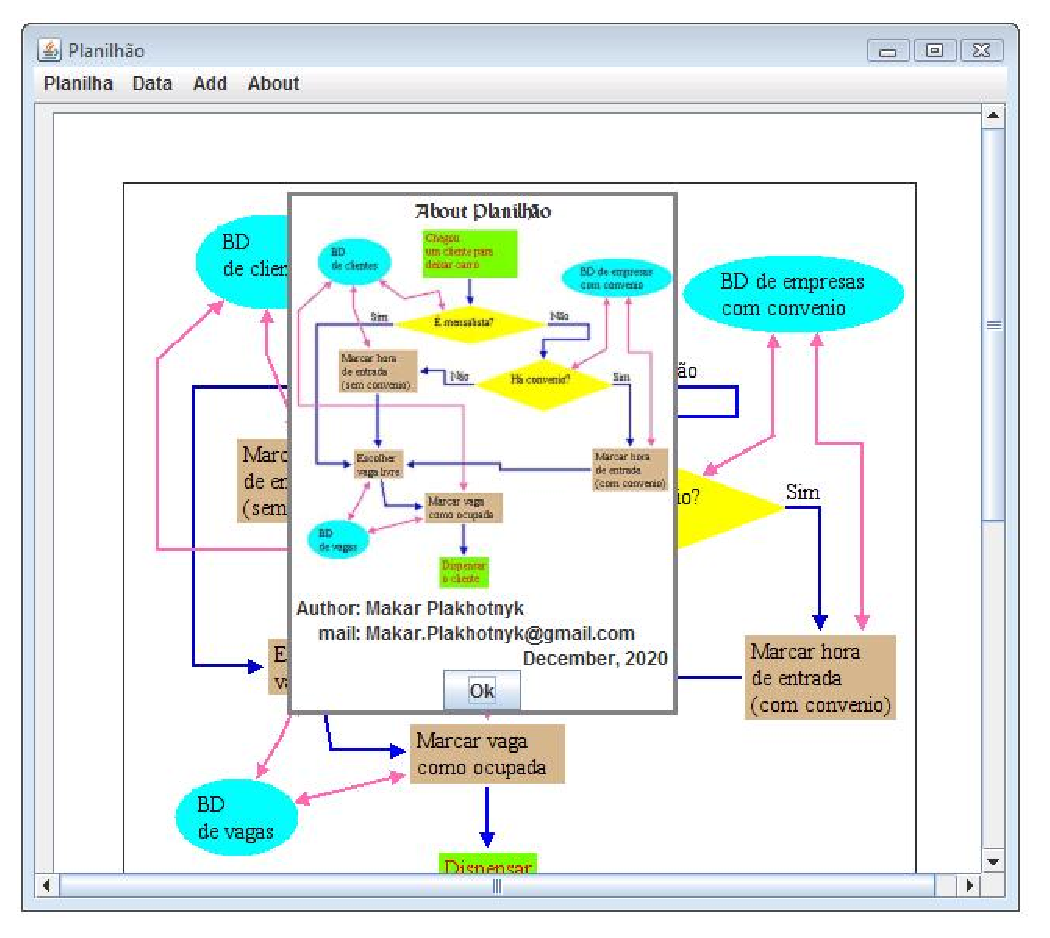
\includegraphics{image-06}
\end{center}
\caption{Frame ``About''}
\end{figure}





\begin{thebibliography}{00} %Exemplos de refer�ncias. Retirar esta se��o, se for o caso.

\bibitem{fonts}
Font metrix, na pagina de Kansas State University.\\
http://faculty.salina.k-state.edu/tmertz/Java/072graphicscolorfont/05fontmetrics.pdf
Acesso: 10/11/2020 07h30m.

\bibitem{itext}
Bruno Lowagie, iText in Action Second Edition. Manning
Publications Co, (2011). ISBN: 978-19-35182-61-0.

\bibitem{cores}
The Other RGB Color Chart (January 2003).\\
http://www2.arnes.si/\~gljsentvid10/barve\_rgb\_xy.html Acesso:
%http://www2.arnes.si/~gljsentvid10/barve_rgb_xy.html 10/11/2020
07h15m.

\end{thebibliography}

\end{document}
